\documentclass{sig-alternate}


\usepackage{graphicx}
\usepackage{amssymb}
\usepackage{epstopdf}
\usepackage{algorithmic}
\DeclareGraphicsRule{.tif}{png}{.png}{`convert #1 `dirname #1`/`basename #1 .tif`.png}

\conferenceinfo{SIGMOD}{'10 Indianapolis, IN}

\title{Streamlining Data Warehousing through Compilation}
\numberofauthors{3}
\author{}%Oliver Kennedy, Yanif Ahmad, Christoph Koch}
%\date{}                                           % Activate to display a given date or no date

\toappear{}

\newtheorem{example}{Example}

\begin{document}

\maketitle
%\section{}
%\subsection{}

\abstract{
In this paper we present SpreadDB\footnote{The name ``SpreadDB" is anonymized for double-blind reviewing}, a compiler for producing customized data warehouses.  SpreadDB uses a novel set of techniques to compile the execution of complex queries down to simple message-passing operations between a set of map datastructures.  By expressing the query result in terms of a recursively defined view-maintenence problem, the data warehouse is able to maintain a set of intermediate results that make it possible to incrementally update the data warehouse in realtime.  The intermediate results produced by these incremental updates can also be used to simplify processing of OLAP-style queries.  Furthermore, the ease of partitioning and distributing SpreadDB's map datastructures makes it feasible to deploy the entire data warehouse in-memory.  The result is a power-efficient data warehousing infrastructure that can maintain synchronization with a relational database, allowing online processing of high-volume aggregate queries.
}
\section{Introduction}

As computer memory grows with respect to the size of data warehouses, the notion of an entirely in-memory data warehouse has become not just feasible, but appealing.  Such a facilty would not only have lower response latency than a comparable disk-based one - especially for queries with random-access patterns, but would be free of the maintenence\cite{}, cooling\cite{}, and power\cite{1154557} costs associated with hard drives.  Moreover, by keeping data entirely in-memory, large datastructures meant to streamline read accesses from disk are not required; Persistence, if required, can be achieved with minimal storage space simply by logging updates.

This paper presents SpreadDB, a system for pushing OLAP precomputations into the cloud; SpreadDB automates the process of creating, loading, and managing in-memory data warehouse infrastructures.  Using a compiler that translates ordinary SQL queries down a simple read/write message-passing model, SpreadDB distributes both processing and storage involved in very large queries.  For example, SpreadDB can compute and distribute the results of a denormalization query.  Thanks to a novel recursive query subdivision technique, the compiler's output is also able to incrementally maintain the query output, keeping the data warehouse constantly synchronized with the source data.

SpreadDB targets OLAP applications that perform real-time analytics of transactionally maintained and/or streaming data.  By feeding it an SQL query, SpreadDB's infrastructure becomes linked to a set of tables in a relational database.  SpreadDB denormalizes the relevant portions of the database, and keeps the denormalized copy synchronized using only a stream of updates to the individual input relations.  

All state in SpreadDB is stored in memory rather than on disk, so not only can complete table scans be completed quickly, but index structures can be simpler and more efficient.  Because the query results are already partitioned across nodes in the warehouse, the work of processing queries can be farmed out as well.  Moreover, the datastructures already used to store intermediate query results bear many similarities to those used by datacube\cite{datacube} implementations and can be used to further simplify the process of aggregation and projection.  Combining these features with its ability to synchronize with an underlying relational database in real time, SpreadDB is able to efficiently process OLAP queries on live transactional data. 

The detailed technical contributions of this paper are as follows.
\begin{itemize}
\item We present SpreadDB, a system for constructing in-memory data warehouse infrastructures that support OLAP queries on high volumes of transactional or streaming data in real-time.

\item We describe the SpreadDB infrastructure, and show how it can be used to efficiently distribute the processing and storage requirements of a large data warehouse.

\item We describe the SpreadDB compiler and show how, using a novel recursive compilation technique, it reduces large join/group by SQL queries down to an extremely straightforward and parallelizable message-passing model. 

\item We show evidence for the scalability of the SpreadDB model by examining SpreadDB's performance on examples drawn from the TPC-H\cite{tpch2008} decision support query benchmark. 
\end{itemize}

\begin{example}\textit
As a running example in this paper, we will use a datacube construction query (shown in Figure \ref{fig:example}) that joins three tables: one storing customer information, one storing orders placed by those customers, and one storing each order's individual line items.  The resulting datacube analyzes the interactions between the way each item was shipped, each customer's nation of origin, the order's priority, and whether the item's arrival and shipping times were late.
\end{example}


\begin{figure}
\begin{center}
\textbf{Schema}
\end{center}
\begin{algorithmic}
\STATE \textbf{create table} customers(cid \textit{int}, nation \textit{int}); 
\STATE \textbf{create table} orders(
\STATE \hspace*{0.1in} oid \textit{int}, o\_cid \textit{int}, opriority \textit{int}, spriority \textit{int},
\STATE \hspace*{0.1in}  \textbf{foreign key}(o\_cid) \textbf{references} customers(cid)
\STATE );
\STATE \textbf{create table} lineitems(
\STATE \hspace*{0.1in} l\_oid \textit{int}, lateship \textit{int}, latedelivery \textit{bool}, shipmode \textit{bool},
\STATE \hspace*{0.1in} \textbf{foreign key}(l\_oid) \textbf{references} orders(oid)
\STATE );
\end{algorithmic}
\begin{center}
\textbf{Query}
\end{center}
\begin{algorithmic}
\STATE \textbf{select} count(*),
\STATE \hspace*{0.1in} nation, cid, oid, opriority, spriority, 
\STATE \hspace*{0.1in} lateship, latedelivery, shipmode 
\STATE \textbf{from} customers, orders, lineitems 
\STATE \textbf{where} o\_cid=cid and l\_oid=oid 
\STATE \textbf{group by cube} 
\STATE \hspace*{0.1in} nation, cid, oid, opriority, spriority, 
\STATE \hspace*{0.1in} lateship, latedelivery, shipmode;
\end{algorithmic}
\caption{An example query that constructs a warehouse for analyzing customer behavior with respect to shipping.  Given a table of customers, orders, and lineitems in those orders, the query builds a datacube over the full join of those tables.}
\label{fig:example}  
\end{figure}

The remainder of this paper is organized as follows.  Section \ref{sec:relatedwork} discusses prior work in the field of OLAP query processing.  In Section \ref{sec:architecture}, we provide an overview of SpreadDB's online infrastructure and discuss how data is managed within that infrastructure.  Section \ref{sec:architecture} describes the offline compilation process used to manage and optimize SpreadDB.  Section \ref{sec:experiments} presents a series of experiments that demonstrate the viability and scalability of in-memory data warehouses.  Finally, Section \ref{sec:optimizations} discusses a set of optimizations provoked by our experiments.  The paper concludes with Section \ref{sec:conclusions}

\section{Related Work}
\label{sec:relatedwork}

\section{Architecture}
\label{sec:architecture}
\begin{figure}
\begin{center}
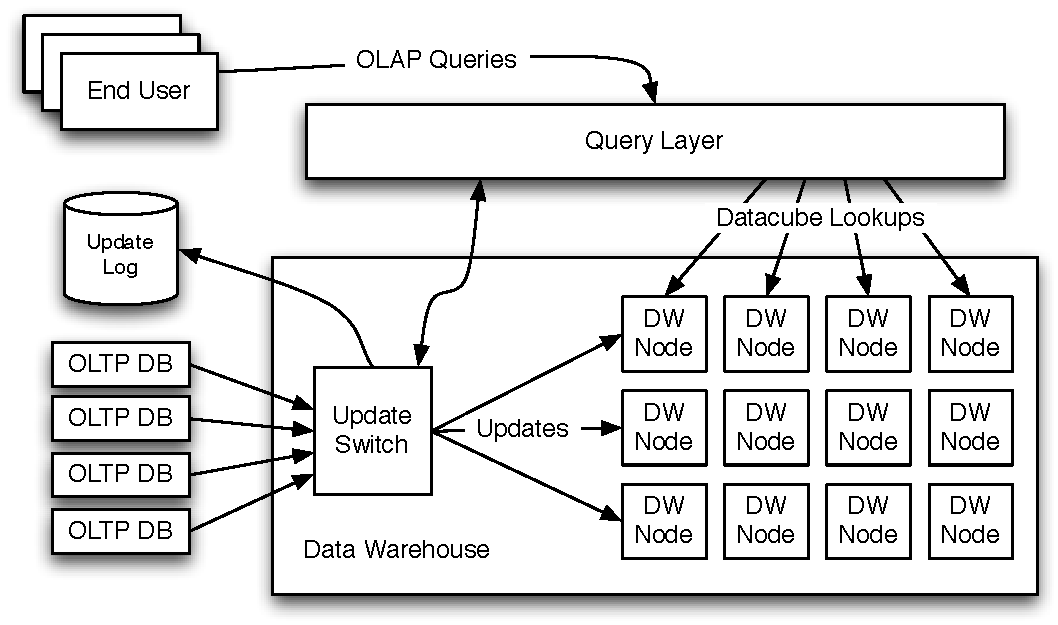
\includegraphics[width=3in]{images/Architecture.pdf}
\caption{SpreadDB's architecture.}
\label{fig:arch}
\end{center}
\end{figure}
SpreadDB consists of three components: a runtime, a \textit{Query Layer}, and a compiler.  A diagram of this architecture is presented in Figure \ref{fig:arch}.  The warehousing runtime accepts relation updates at a coordinator node called the \textit{Switch}, and distributes their data throughout an array of data warehouse storage nodes, or \textit{DW Nodes}.  Though this paper focuses on a runtime with a centralized switch, we discuss a distributed switch implementation in Section \ref{sec:distswitch}.

Adjacent to the runtime is the \textit{Query Layer}, a component that acts as an intermediary between the end user and the dw nodes.  The query layer accepts roll-up and drill-down queries, translates them into the corresponding set of data warehouse lookups, and executes those queries on the warehouse.

SpreadDB's final component is a compiler that guides the behavior of the other three components.  The SpreadDB compiler takes schemas for one or more input relations and an arbitrary SQL query as input.  The query is decomposed into a set of subqueries, each representing a join over some subset of the input relations.  Each subquery is materialized into a \textit{map}, that is partitioned across the DW nodes.  

Based on these subqueries, the compiler generates a series of \textit{update rules} that translate changes in the input relations to map deltas.  These update rules take the form:
$$+R(x_1, x_2, x_3, \ldots)\ :\ Map\ K[\ldots]\ += Expression$$
That is, when the tuple $(x_1, x_2, x_3, \ldots)$ is inserted into input relation $R$, adjust the target map $K$ by the indicated arithmetic expression over constants, variables ($x_n$), or the contents of other maps.  
 
It is possible for an update rule to modify an an entire cross section of a map.  Such updates are expressed via variables in the update rule not bound to one of the input parameters.  We refer to these as loop variables.  A loop variable occurs exactly twice in an update rule, once as a key in the target map, and once as an key for a map in the expression.  Thus an update rule with loop variables behaves as if it were a set of parallel updates; every update corresponds to one possible valuation of all loop variables selected from the domains of the map they index into.

When a tuple is added to or removed from an input relation, the Switch composes a set of messages parametrized on the tuple's contents and dispatches them into the data warehouse as a sequence of map reads and writes.  Nodes being read from accept and process the requests and forward the responses to the appropriate writers.  We refer to this entire sequence of operations as an update.

\begin{example}
One of the rules the compiler generates for updates to the lineitems table in the example datacube is
{\footnotesize
\begin{eqnarray*}
+lineitems(l\_oid,lateship,latedeliver,shipmode) : \\
Map\ 1[shipmode,latecommit,lateship,spriority,\\ opriority,l\_oid,cid,nation] \\
 += Map\ 5[cid,nation,l\_oid,opriority,spriority]
\end{eqnarray*}}
\noindent Here, Map 1 represents the query output $count(*)$, while Map 5 represents the natural join $customers \bowtie orders$\footnote{Map 5 actually represents the $count(*)$ of the join, grouped by all columns.  However, because $cid$ and $oid$ are keys for each input table, the count is binary; Each entry in Map 5 is either 0 or 1.  It is also possible to treat Map 5 as a map from $(cid,oid)$ to $\{(nation, opriority, spriority)\}$. }.  Note that the variables $cid$, $nation$, $opriority$, and $spriority$ do not appear in the input tuple.  These variables are treated as loop variables; an entire cross-section of Map 1 will be updated by the values stored in the corresponding portion of Map 5.  

The update corresponding to this rule is coordinated by a subset of nodes that store partitions of Map 1.  Each node coordinates updates only for those partitions it stores locally.  Simultaneously, read requests are dispatched by the switch to a subset of the nodes managing partitions of Map 5, and the responses are forwarded to the appropriate Map 1 nodes.  
\end{example}

\subsection{Anatomy of an Update}

\begin{figure}
\begin{center}
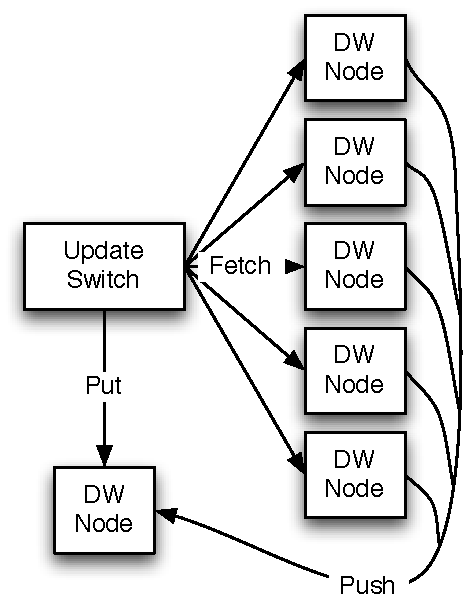
\includegraphics[width=1.5in]{images/UpdateStep.pdf}
\caption{Information flow during one map update.}
\label{fig:updatestep}
\end{center}
\end{figure}

A map update begins at the Switch when an input table is modified.  Each input table is associated with one or more triggers, each requiring a write to some range of map values and zero or more reads from different maps.  For each trigger, the Switch identifies and sends a PUT message to each DW Node managing a map being written to.  Additionally, the Switch identifies all DW Nodes managing maps that will be read from and sends a FETCH message to them, requesting the desired map values.  Finally, if required (i.e., if SpreadDB is being used standalone, without an underlying database), the switch can log the update to disk for persistence.

The nodes receiving a FETCH request perform the appropriate reads and send their responses to the PUT nodes in a PUSH message.  Upon receipt of all necessary PUSH messages, the PUT nodes compute the update expression and modify the affected maps.  An illustration of the complete message-passing process is presented in Figure \ref{fig:updatestep}.  

\subsubsection{Trigger Dispatch}
Maps are partitioned along dimensional axes when they grow beyond the capacity of a single node, akin to the partitioning done in grid files\cite{318586}.  To streamline the dispatch of messages to component nodes, the switch pre-generates a spatial index for each template, similar to the grid file directory.  Every entry in the spatial index contains a set of PUT and FETCH messages.  When the template is triggered, the tuple's values are used to index into the spatial index and the corresponding messages are parametrized and sent.  The algorithm for generating the spatial index is presented in Figure \ref{alg:dispatch}.

\begin{figure}
\begin{algorithmic}[1]
\STATE $Msgs \leftarrow \emptyset$
\FORALL{Update $U \in$ Trigger}
	\STATE Region $Reg = \pi_{U.target.loop\_vars} \left(index(U.target\_map)\right)$
	\FORALL{Partition $\{P | P\in U.target\_map \wedge (P \cap Reg \neq \emptyset)\}$}
		\STATE $Reads = \emptyset$
		\FORALL{Ref $R \in get\_map\_refs(U.expression)$}
			\STATE $RReg \leftarrow \pi_{R.loop\_vars} P$
			\STATE $RPart \leftarrow \{RP | RP\in R.map \wedge (RP \cap RReg \neq \emptyset)\}$
			\STATE $Reads \leftarrow Reads \cup \{(ReadP.node, R)\}$
		\ENDFOR
		\STATE $Reads \leftarrow group\_by\_node(Reads)$
		\STATE $Msgs \leftarrow put(U, P, Reads.size)$
		\FORALL{$($Node $N, \{$Ref $R\}) \in Reads$}
		  \STATE // PUSH results to $P.node$
			\STATE $Msgs \leftarrow fetch(N, \{R\}, P.node)$
		\ENDFOR
	\ENDFOR
\ENDFOR
\end{algorithmic}
\caption{The Switch's trigger dispatch algorithm}
\label{alg:dispatch}
\end{figure}

Looping updates require the Switch to match corresponding read and write partitions.  The correspondence is obtained by identifying intersections between partitions of the target map that are affected by the update, and those of each map in the update expression.  This is equivalent to a join over components of the spatial index stored at the Switch.  Loop-free updates are a special case of this, where only one partition is required from each map.  The trigger dispatch algorithm is shown in Figure \ref{alg:dispatch}.

\subsubsection{Get Collation}

FETCH responses, or PUSH messages for an update are sent to the node managing the partition being updated.  Having received the number of FETCH messages sent by the switch with the PUT message, the destination node can buffer PUSH messages until all have arrived.  At this point, if the update is loop-free, the destination node simply uses the contents of the PUSH messages to evaluate the update expression.

\begin{figure}
\begin{algorithmic}[1]
\STATE Given: Update $U$
\FORALL{Ref $R \in U.expression$}
	\STATE $Inputs \leftarrow Inputs \cup (R, \emptyset)$
\ENDFOR
\FORALL{$($Ref $InR,$ Value $V) \in \cup(msg_{PUSH})$}
	\FORALL{$(R, Table) \in Inputs$}
		\IF{$check\_match(InR, R)$}
			\STATE $Table \leftarrow Table \cup (InR.keys, V)$
		\ENDIF
	\ENDFOR
\ENDFOR
\FORALL{$(K,\{V\}) \in $ JOIN $ (Keys, Val) \in Inputs$}
	\STATE $Target = bind\_vars(U.target \leftarrow Keys)$
	\STATE $apply(Target, bind\_vars(U.expression \leftarrow \{V\}))$
\ENDFOR
\end{algorithmic}
\caption{The DW Node's collation algorithm}
\label{alg:collation}
\end{figure}

If the update requires a loop, the destination node must do some processing.  The node first generates a set of tables, one for each map reference in the update expression.  Arriving map values populate tables that correspond to any map reference matching the value's keys, where loop variables act as wildcards.  When all values have been received, the destination node computes the natural join of all of the generated tables, effectively producing one update value for every assigned value in the domain of all of the loop variables.  The loop-free update is a special case of this where each generated table contains only one row.  The collation algorithm is shown in Figure \ref{alg:collation}

\subsection{Consistency Model}

The materialize

SpreadDB's update delta-encoding uses materialized subqueries already stored within the warehouse to perform updates.  This dependency requires that all reads see a consistent snapshot of the warehouse at the completion of the previous update.  Thus, all reads and writes must be executed as if there were a total ordering over all updates.  As the clearinghouse for updates, the Switch presents an ideal point for generating this ordering.  

Every update is assigned a version number by the switch as it is issued.  The 
As they are 

Every update is assigned a version number by the switch.  The maps that each update modifies and reads are known.  The switch maintains a list of modification times for each partition in the warehouse.  With each request to the DW Nodes, the switch attaches a version 

 first looks up the most recent modification time for each get required by the update, and subsequently updates the modification times for each put required by the update.  

When applying gets, each warehouse node first ensures that it has successfully applied all requests prior to the indicated version number.  A short history of prior incarnations of each partition are also maintained in case a get arrives after a subsequent put.  Each put also includes the version number of the last fully completed update.  This allows the target node to discard old incarnations of the partition.

Some trickery will be required to get this table into the middleware.  Perhaps the switch can periodically broadcast it over?

\section{Compilation}
\label{sec:compilation}

\subsection{Update Rules}
- Translating SQL into Update Rules

- Update DAGs/Data flow graphs

- Exploiting Foreign Keys

- Cascading Map Rejection

\begin{figure}
\begin{center}
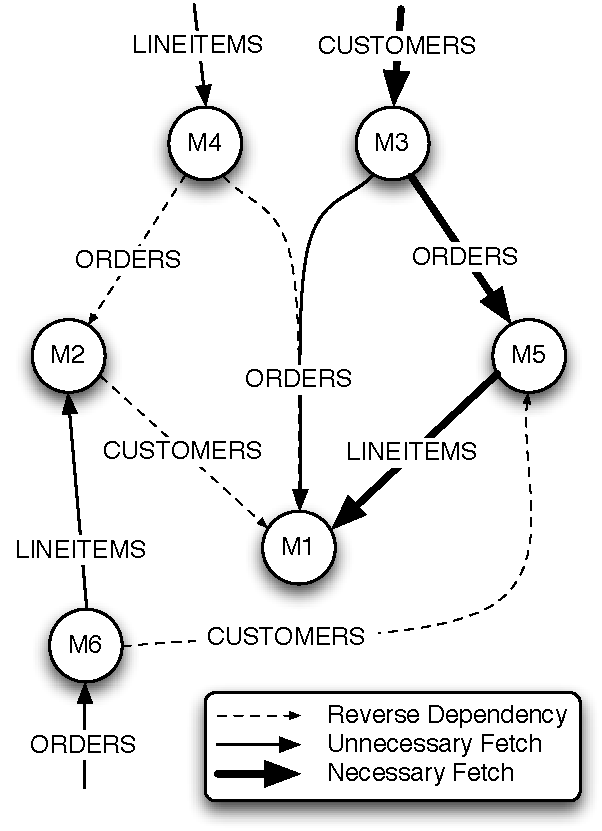
\includegraphics[width=2.5in]{images/q12_graph.pdf}
\caption{Data-flow graph for the example query.  Light and dashed edges can be optimized out, given cascading delete foreign key constraints.}
\label{fig:dataflow}
\end{center}
\end{figure}

\subsection{Layout}
How do we partition data (the layout)?  Where do various bits of code get executed live?  What kind of runtime analytics do we need to collect to manage the data layout on the fly? 


\section{Experiments}
\label{sec:experiments}

\section{Optimizations}
\label{sec:optimizations}

\subsection{Distributing the Switch}
\label{sec:distswitch}
The role of the switch is to provide a synchronization mechanism for the updates.  Specifically, the delta encoding approach used by the update rules requires that all update rules be applied to a consistent snapshot of the maps.  The current implementation of SpreadDB performs this synchronization at a single node.  However, limiting the switch to only one node creates a scaling bottleneck.  

Despite the cloud computing mantra of rejecting consistency, this application requires it.  Complex locking protocols have poor scaling performance, so a simpler, lock-free protocol is required.  We achieve this goal by introducing the notion of \textit{pipeline scheduling}.  Pipeline scheduling exploits the acyclicity of compiler-generated data-flow graphs to allow nodes to correctly interleave and process update rules with only limited network overhead and processing latency.

\subsection{Pipeline Scheduling}
Loose clock synchronization between nodes is assumed, and allows time to be partitioned into a sequence of numbered ticks, each lasting on the order of seconds.  When a set of updates is triggered, a switch node sends tentative put requests to all participating nodes.  These nodes respond with their current tick counter, and the switch forwards the maximum returned tick to all nodes.

The updates are considered to have been posted at the maximum returned tick.  However processing is deferred for a number of ticks equal to the depth of the map being updated.  The result is a data-flow process resembling a parallelized CPU pipeline.

During a given tick, all updates scheduled for processing are evaluated.  Once all updates scheduled for the tick have completed, the node responds to FETCH requests for the tick with PUSH messages.  Recall that each edge in the data flow graph represents a FETCH request for a specific update.  The difference in depth between the edge's ends is the number of ticks in advance of the PUT that the response is sent.  

For example, in Figure \ref{fig:dataflow} without removing any edges, $Depth(M1) = 2$, $Depth(M2) = 1$, and $Depth(M4) = 0$.  Updates to map $M1$ scheduled for processing during tick 4 would receive data from map $M2$ during tick 3, and from map $M1$ during tick 2.

%\subsection{Synchronizing Ticks}
%Ensuring that nodes are operating on the same tick poses two challenges.  First, the nodes must 
%
%Clock tick synchronization requires two pieces of functionality: Asserting 
%
%Loose clock tick synchronization requires two stages.  
%
%is achieved through a cascading gossip protocol.
%
%
%\subsection{Distributed Queries}
%

\section{Conclusions}
\label{sec:conclusions}

\bibliographystyle{abbrv}
\bibliography{spread}




%\begin{figure}
%\begin{center}
%\begin{itemize}
%\item Middleware
%\begin{itemize}
%\item Query(Query) 
%\end{itemize}
%
%\item Warehouse Nodes
%\begin{itemize}
%\item Get(\{Entry\}, Version)
%\item Fetch(\{Entry\}, Version, Destination)
%\item Push(\{(Entry, Value)\}, Version)
%\item Put(Template, \{Params\}, Version [, Fetches])
%\end{itemize}
%
%\item Switch
%\begin{itemize}
%\item update(Relation, \{Params\})
%\end{itemize}
%
%\end{itemize}
%\caption{SpreadDB's API}
%\label{fig:api}
%\end{center}
%\end{figure}

\end{document}  